\documentclass[border=4pt]{standalone}
\usepackage{tikz}
\usetikzlibrary{shapes.symbols,positioning}

\begin{document}
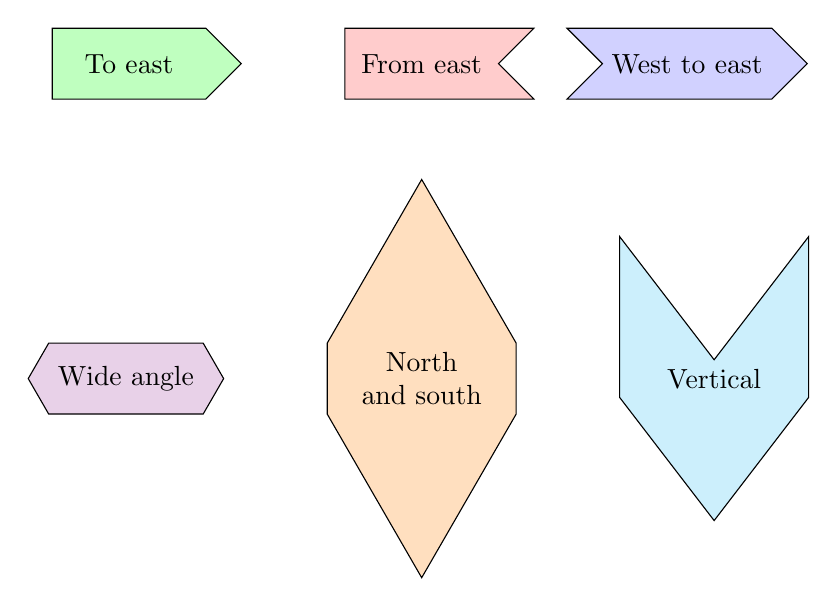
\begin{tikzpicture}[
  every node/.style={signal,draw,minimum width=24mm,minimum height=9mm,align=center},
  node distance=10mm and 13mm
]
  \node[signal to=east,fill=green!25] (to) {To east};
  \node[signal to=nowhere,signal from=east,fill=red!20,right=of to] (from) {From east};
  \node[signal from=west,signal to=east,fill=blue!18,right=of from] (through) {West to east};

  \node[signal to=north and south,signal pointer angle=60,fill=orange!25,
    below=of from] (vertical) {North\\and south};
  \node[signal to=east and west,signal pointer angle=120,fill=violet!18,
    left=of vertical] (wide) {Wide angle};
  \node[signal from=north,signal to=south,signal pointer angle=75,fill=cyan!20,
    right=of vertical] (verticalthrough) {Vertical};
\end{tikzpicture}
\end{document}
